\documentclass[11pt,a4paper,twocolumn]{article}
\usepackage[utf8]{inputenc}
\usepackage[T1]{fontenc}
\usepackage{times}
\usepackage[left=1.5cm,top=1.5cm,right=1.5cm,bottom=2cm]{geometry}
\usepackage{amsmath}
\usepackage{amssymb}
\usepackage{makeidx}
\usepackage{graphicx}
\usepackage{hyperref}
\usepackage[portuguese]{babel}
\title{\textbf{Diodos aplicados à sensores digitais de imagem}}
\author{Leandro Assis dos Santos}

\begin{document}
\maketitle

\section*{Introdução}
		Sensores digitais de imagem são sensores que transdutam a intensidade luminosa incidente sobre eles em sinais elétricos analizáveis por um sistema computacional. Esses sensores são usados em imagens eletrônicas aplicadas a diversos dispositivos como câmeras digitais, mouses ópticos, equipamentos de imagem médica, equipamentos de visão noturna e térmica, LIDARs (Light Detection and Ranging), dentre outros.
				
		Os sensores de imagem são feitos de fótodiodos, que é um tipo de diodo construído de forma a possibilitar a utilização da incidência de luz como fator determinante no controle da corrente elétrica, e um ou mais transistores ativos. Ou seja, os fótons incidentes sobre o sensor interagem com o fótodiodo para mover elétrons de forma proporcional ao aumento da intensidade luminosa no cristal, juntamente a isso os transistores atuam de forma programada, como será visto mais a frente, a fim de registrar a imagem,. Os sensores modernos de imagem utilizam da exploração desse efeito fotoelétrico concomitantemente da característica capacitiva que junções pn em polarização reversa (fótodiodos em polarização reversa) possuem. 
		
		Em resumo, ao polarizar um diodo reversamente com uma fonte de tensão $V_{R}$ (Figura 1), o campo elétrico interno da junção pn que constitui o diodo é reforçado. Por conta disso, a barreira de potencial se fortalece e mais íons (de ambos, aceitadores e doadores) ficam expostos. Devido ao campo induzido pelo terminal negativo da fonte $V_{R}$, as lacunas da região p são atraídas para o extremo do ânodo do diodo, e de forma similar (mas por conta do campo induzido pelo terminal positivo) os elétrons são atraídos para o extremo do cátodo do diodo.
		
		\begin{figure}[!h]
			\centering
			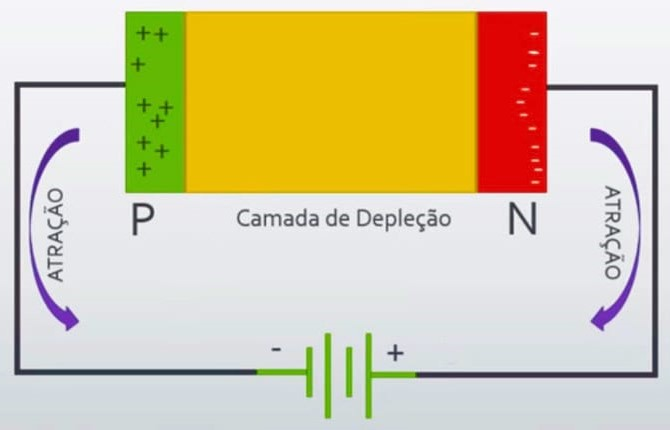
\includegraphics[scale=0.3]{imagens/diodo_polarizado_reversamente.jpg}
			\caption{Diodo polarizado reversamente.}
		\end{figure}
		Em razão da concentração de cargas nos extremos do diodo e do aumento da barreira de potencial, isto é, o aumento da voltagem entre as extremidades da região de depleção, a região de depleção se torna mais larga e podemos pensar nos extremos do diodo como as placas de um capacitor. A junção pn portanto, quando polarizada reversamente, possui capacitância dependente de $V_{R}$.
		
		Uma vez que possui-se o fótodiodo funcionando como um capacitor sob uma tensão reversa, o dispositivo se carregará com um dado valor $V_{C}$ que depende do tempo ao qual o fótodiodo (agora agindo como capacitor) ficou alimentado pela tensão reversa $V_{R}$. Com o fótodiodo carregado permite-se a entrada de luz sobre o sensor, que resultará em uma indução de corrente na junção pn e, consequentemente, em uma diminuição na tensão $V_{C}$. A partir da observação individual da tensão $V_{C}$ em uma matriz de fótodiodos é possível fazer a transdução da luz incidente sobre o sensor em uma imagem.
		
\section*{Tipos de sensores de imagem}
		Os sensores de imagem podem ser separados em dois principais tipos, eles são os CCDs (\textit{Charge-Couple Device}) e os sensores CMOS, configurações de sensores baseados em APS (\textit{Active Pixel Sensor}), estes podendo ser classificados de acordo com o número de transistores por pixel, como por exemplo 3T-APS, 4T-APS e assim por diante. Ambos os dispositivos são feitos com tecnologia MOS (\textit{Metal Oxide Semiconductor}), com CCDs baseados em capacitores MOS e os sensores CMOS baseados em amplificadores MOSFET. A seguir entra-se em mais detalhes sobre cada tipo de sensor, suas características, histórias, vantagens e desvantagens.
		
	\subsection*{A história dos sensores de imagem}
		Os sensores CCDs são pioneiros no ramo de imagem digital e sua origem remonta às pesquisas com tecnologia MOS de Willard Boyle e George E. Smith. Durante a pesquisa descobriram que uma carga elétrica poderia ser armazenada em pequenos capacitores MOS, descoberta essa que se tornou a base para o sensor CCD, inventado em 1969.
		
		Apenas em 1980 surgiu um fator chave para os sensores CMOS modernos, o fótodiodo ``fixado'' (do inglês PPD - Pinned PhotoDiode) inventado por Nobukazu Teranishi, Hiromitsu Shiraki e Yasuo Ishihara. O diferencial desse componente em relação aos demais é o baixo \textit{lag}, baixo ruído, alta eficiência quântica (taxa de conversão de fótons em elétrons) e baixa corrente quando aplicado a pouca luminosidade. A partir de 1987, os PPDs começaram a ser incorporados na maioria dos sensores CCDs, e desde então são usados em todos os sensores CCD e CMOS.
	
		Apesar dos sensores CCDs terem sido pioneiros no ramo de medição científica nos anos 80 e se tornado o sensor de escolha para praticamente toda aplicação de imagens nesta época, o desenvolvimento de sensores CMOS atingiu um ponto em que começou a substituir os sensores CCDs em aplicações de baixa performance. Com o passar do tempo os sensores de tecnologia CMOS se expandiram, enquanto os de tecnologia CCD estagnaram. De forma geral, ambos os dispositivos são utilizados de acordo com a necessidade da aplicação.
		
	\subsubsection*{Sensores de Pixel Passivo - PPS} 
		Os precursores dos sensores APS foram os PPS (do inglês, passive-pixel sensor), um tipo de matriz de pixels formada por fótodiodos e uma chave MOSFET, que consiste em ``pixels passivos'' sem amplificação, ou seja, essa configuração de pixel transfere diretamente o sinal acumulado para fora do pixel. Nesses sensores cada pixel possui uma junção pn, capacitor integrado e transistores de seleção. Essa configuração de pixels passivos foi proposta por G. Weckler em 1968 e antecedeu a criação dos CCDs. Os PPS sofrem de diversas limitações como alto ruído, baixo tempo de leitura e dificuldade de escalabilidade. De forma geral, os sensores CCDs possuem matrizes de pixels passivos.
		
	\subsubsection*{Sensores de Pixel Ativos - APS}
		Esses sensores consistem de ``pixels ativos'', que consiste em um ou mais amplificadores MOSFET que convertem a carga fótogerada em uma tensão, amplifica o sinal de tensão e reduz o ruido. Esse conceito de pixel foi proposto por Peter Noble em 1968, entretanto esta topologia de pixels só foi fabricada a partir de 1985 devido as evoluções nos processos de fabricação dos transistores MOS.  Os sensores CMOS utilizam dessa configuração de pixels para seu funcionamento, tendo como principal diferença o uso de transistores CMOS ao invés de transistores PMOS ou NMOS.
	
	\begin{figure}[!ht]
		\centering
		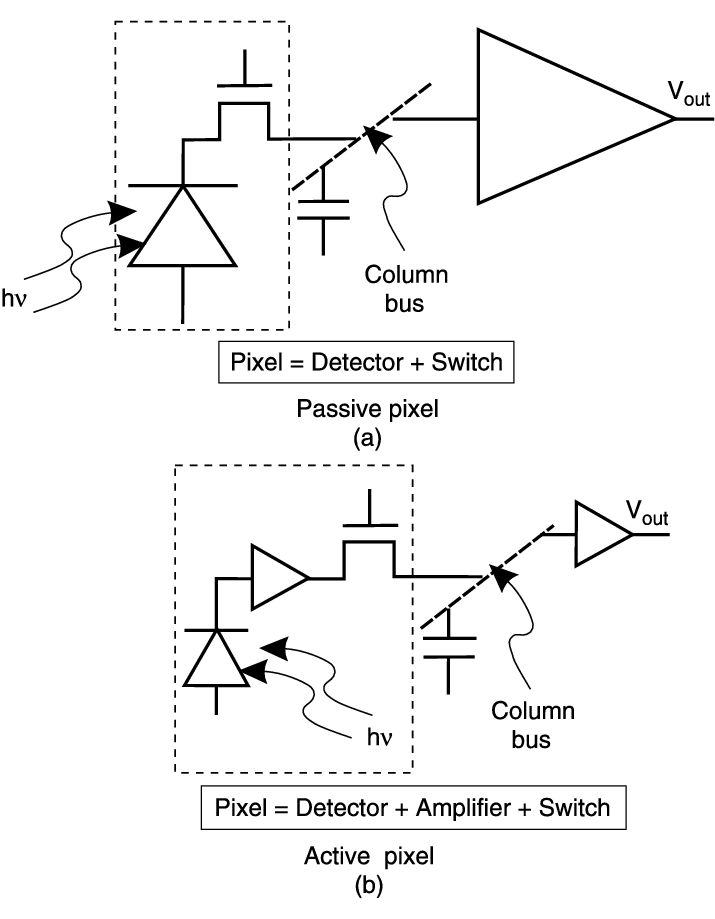
\includegraphics[scale=0.26]{imagens/passive_vs_active.png}
		\caption{Apresentação das configurações de PPS (a) e APS (b).}
	\end{figure}
	
	\subsection*{Sensores CCD}
	Como dito anteriormente, os CCDs são circuitos integrados formado por pixels feitos de silício. Esses pixel dispostos em colunas possuem um \textit{gate} responsável por controlar o deslocamento e armazenamento de cargas através da tensão, a Figura 3 apresenta a transição de cargas de pixels de colunas adjacentes feito ao comutar o gate da coluna de destino para HIGH e da coluna de partida para LOW de forma gradativa.
	
	\begin{figure}[!ht]
		\centering
		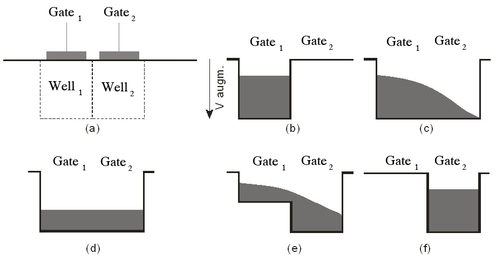
\includegraphics[scale=0.52]{imagens/ccd.jpg}
		\caption{Fluxo de carga de pixels adjacentes.}
	\end{figure}
		
	Como apresentado de forma gráfica em \cite{Spectral}, o funcionamento dos CCDs pode ser descrito, de forma análoga, como uma matriz de baldes (pixels) coletando água da chuva (fótons). Os baldes são expostos à chuva pela mesma quantidade de tempo, e consequentemente se enchem com diferentes quantidades de água. A seguir o CCD inicia a leitura de cada balde por vez. Este processo de leitura é feito transferindo a água de cada balde, da coluna mais a esquerda para o balde adjancente em uma coluna vazia ao lado. Essa coluna anteriormente vazia desloca um de seus baldes para baixo por vez, onde se encontra um conversor que reconhece e armazena o nível d'água. Ou seja, há um deslocamento horizontal dos ``baldes'' de uma coluna para ``baldes"" de outra, e posteriormente um deslocamento vertical de um ``balde'' por vez na coluna de saída.
	
	Na prática, como apresentado na Figura 4, o fótodiodo (polarizado reversamente) de cada pixel é exposto aos fótons incidentes sobre o sensor. Devido ao fluxo de fótons sobre o fótodiodo, elétrons são liberados - proprocionalmente a intensidade e cor da luz - e, consequentemente, lacunas são criadas na estrutura cristalina. Ou seja, há um fluxo de corrente induzido no fótodiodo agindo como capacitor. Inicialmente, esses elétrons ficam desprendidos na camada de depleção, mas posteriormente são concentrados na parte N+ do fótodiodo por conta do potencial positivo que é induzido nesta parte apenas durante a leitura.
	
	Através do acionamento do transistor de seleção pela entrada SEL as cargas na coluna mais próxima ao amplificador ($COL_{j}$) são deslocadas para um registrador de deslocamento, que será responsável por transferir a carga de um pixel da coluna por vez ao amplificador. Devido ao acionamento do transistor de seleção - que age como o \textit{gate} descrito anteriormente-, após  as cargas da coluna serem transferidas para a saída, as cargas na coluna anterior ($COL_{j-1}$) são deslocadas para a coluna $COL_{j}$. O processo segue em \textit{loop} até que todas as linhas e colunas tenham sido iteradas. A leitura das cargas no CCD pode ser feita de forma mais rápida ao construir o CCD com amplificadores em cada vértice da matriz de pixels, e adicionar registradores de deslocamento em cada aresta.
	
	Após o processo, afim de preparar os pixels do CCD para uma nova leitura, o transistor de \textit{reset} é acionado pela entrada RST, e todos os \textit{gates} são levados à nivel lógico alto - entrada SEL acionada para todas os pixels -, fazendo com que os fótodiodos de cada pixel voltem para o estado inicial e fiquem prontos para um novo processo.

	\begin{figure}[!h]
		\centering
		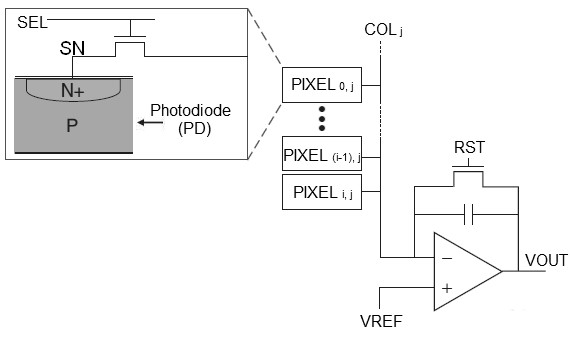
\includegraphics[scale=0.56]{imagens/passive-pixel.jpg}
		\caption{\textit{Array} simplificada de um CCD.}
	\end{figure}
	
	\subsection*{Sensores CMOS}
	Fazer quarta
	\subsection*{CCD vs. CMOS}
	Fazer quarta

	\section*{Simulação de um sensor CMOS simplificado}
	Fazer quinta	
	\section*{Extra: Separação de cores}
	Fazer quinta
	
	\begin{thebibliography}{99}
		\bibitem[1]{MazinSaad2019}
		{Mazin H.; Saad D. {Design and simulation of a CMOS image sensor with a built-in edge detection for tactile vision sensory substituition}, \textbf{AIMS Electronics and Electrical Engineering}. DOI: 10.3924/ElectrEng.2019.2.144, 06 May 2019.}
		
		\bibitem[2]{Spectral}
		{Spectral Instruments, Inc. {What is a CCD?}, Disponível em: \url{https://specinstcameras.com/what-is-a-ccd/}, 2021. Acesso em: 07 mar 2022.}
		
		\bibitem[3]{ImageSensorWiki}
		{IMAGE sensor. In:WIKIPÉDIA: a enciclopédia livre. Wikimedia, 2006. Disponível em: \url{https://en.wikipedia.org/wiki/Image_sensor} Acesso em: 07 mar 2022.}

		\bibitem[4]{ActivePixelWiki}
		{ACTIVE-pixel sensor. In:WIKIPÉDIA: a enciclopédia livre. Wikimedia, 2006. Disponível em: \url{https://en.wikipedia.org/wiki/Active-pixel_sensor} Acesso em: 04 mar 2022.}
		
		\bibitem[5]{StefanoMeroli}
		{Meroli, Stefano, {Design and implementation of Active Pixel Sensors (APS)}, Disponível em: \url{https://meroli.web.cern.ch/lecture_activepixelsensors.html}. Acesso em: 07 mar 2022.}
		
		\bibitem[6]{ColorRecognition}
		{Computerphile, {Capturing Digital Images (The Bayer Filter) - Computerphile}. Youtube, 2015. Disponível em: \url{https://www.youtube.com/watch?v=LWxu4rkZBLw}. Acesso em: 07 mar 2022.}
		
		\bibitem[7]{ColorRecognition}
		{ALL ABOUT ELECTRONICS, {Image Sensors Explained: How CCD and CMOS Sensors works? CCD vs CMOS}. Youtube, 2019. Disponível em: \url{https://www.youtube.com/watch?v=FKJFIzDfUNE&t=421s}. Acesso em: 05 mar 2022.}
		
		\bibitem[8]{ColorRecognition}
		{Hodgins, Sean, {I Made My Own Image Sensor! (And Digital Camera)}. Youtube, 2020. Disponível em: \url{https://www.youtube.com/watch?v=PaXweP73NT4}. Acesso em: 03 mar 2022.}

	\end{thebibliography}
\end{document}